%\documentclass{beamer}
\documentclass[aspectratio=169]{beamer}
\usetheme{Boadilla}
%\usetheme{Warsaw}
%\setbeamercovered{transparent}
\beamertemplatetransparentcoveredhigh
\usepackage[portuges]{babel}
\usepackage[utf8]{inputenc}
\usepackage{lmodern}
\usepackage[T1]{fontenc}
\usepackage{listings}
\usepackage{hyperref} 
\usepackage[portuguese, linesnumbered, vlined, titlenumbered, ruled]{algorithm2e}
\lstset{frame=tb,
  language=C,
  aboveskip=3mm,
  belowskip=3mm,
  showstringspaces=false,
  columns=flexible,
  basicstyle={\small\ttfamily},
  numbers=none,
  breaklines=true,
  breakatwhitespace=true,
  tabsize=3
}

\newcommand{\eng}[1]{\textsl{#1}}
\newcommand{\cod}[1]{\texttt{#1}}

\title[Análise de Algoritmos]{Algoritmos e Estrutura de Dados II}
\subtitle{Análise de Algoritmos}
\author[Frederico Santos de Oliveira]{prof. Frederico Santos de Oliveira}
\institute[UFMT]{Universidade Federal de Mato Grosso\\ Instituto de Engenharia}
\date{}

\begin{document}

%%%%%%%%%%%%%%%%%%%%%%%%%%%%%%%%%%%%%%%%%%%%%%%%%%%%%%%%%%%%%%%%%%%%%%%%%%%%%%%%%%%%%%%%%%%%
\begin{frame}[plain]
  \titlepage
\end{frame}

%%%%%%%%%%%%%%%%%%%%%%%%%%%%%%%%%%%%%%%%%%%%%%%%%%%%%%%%%%%%%%%%%%%%%%%%%%%%%%%%%%%%%%%%%%%%
%\section*{Roteiro}
%%%%%%%%%%%%%%%%%%%%%%%%%%%%%%%%%%%%%%%%%%%%%%%%%%%%%%%%%%%%%%%%%%%%%%%%%%%%%%%%%%%%%%%%%%%%

\begin{frame}
  \frametitle{Agenda}
  \tableofcontents
\end{frame}

%%%%%%%%%%%%%%%%%%%%%%%%%%%%%%%%%%%%%%%%%%%%%%%%%%%%%%%%%%%%%%%%%%%%%%%%%%%%%%%%%%%%%%%%%%%%
\section{Introdução}
%%%%%%%%%%%%%%%%%%%%%%%%%%%%%%%%%%%%%%%%%%%%%%%%%%%%%%%%%%%%%%%%%%%%%%%%%%%%%%%%%%%%%%%%%%%%

\begin{frame}{Introdução}{Algoritmos}
\begin{block}{O que é um algoritmo?}{
Um conjunto de instruções executáveis para resolver um problema.}
\end{block}
\begin{itemize}
\item O problema é a motivação para o algoritmo.
\item As instruções têm de ser executáveis.
\item Geralmente existem vários algoritmos para um mesmo problema. Como escolher?
\item Representação: descrição das instruções suficientes para que o leitor o entenda.
\end{itemize}
\begin{figure}[!ht]
  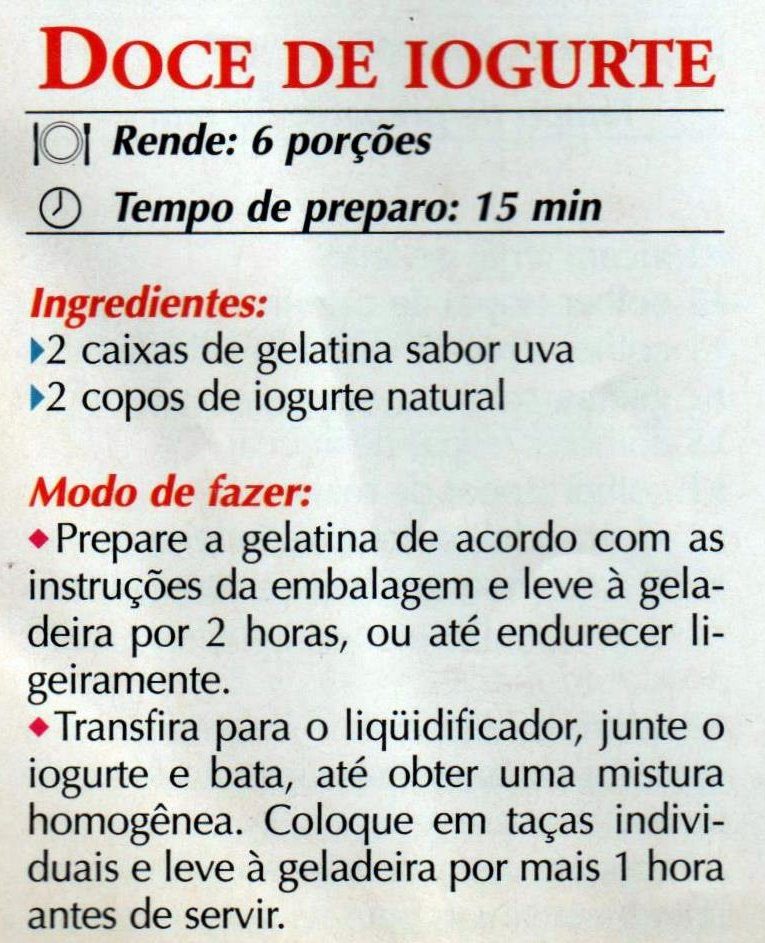
\includegraphics[width=70pt]{imgs/receita.jpg}
  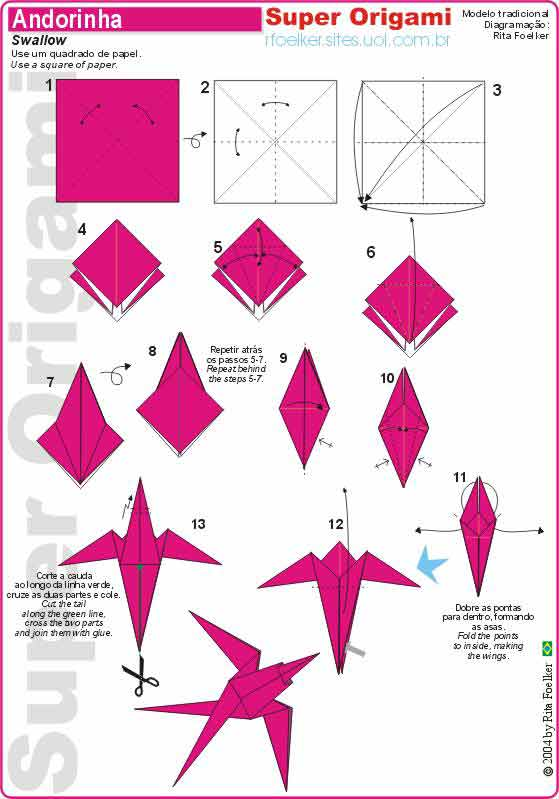
\includegraphics[width=58pt]{imgs/origami.jpg}
  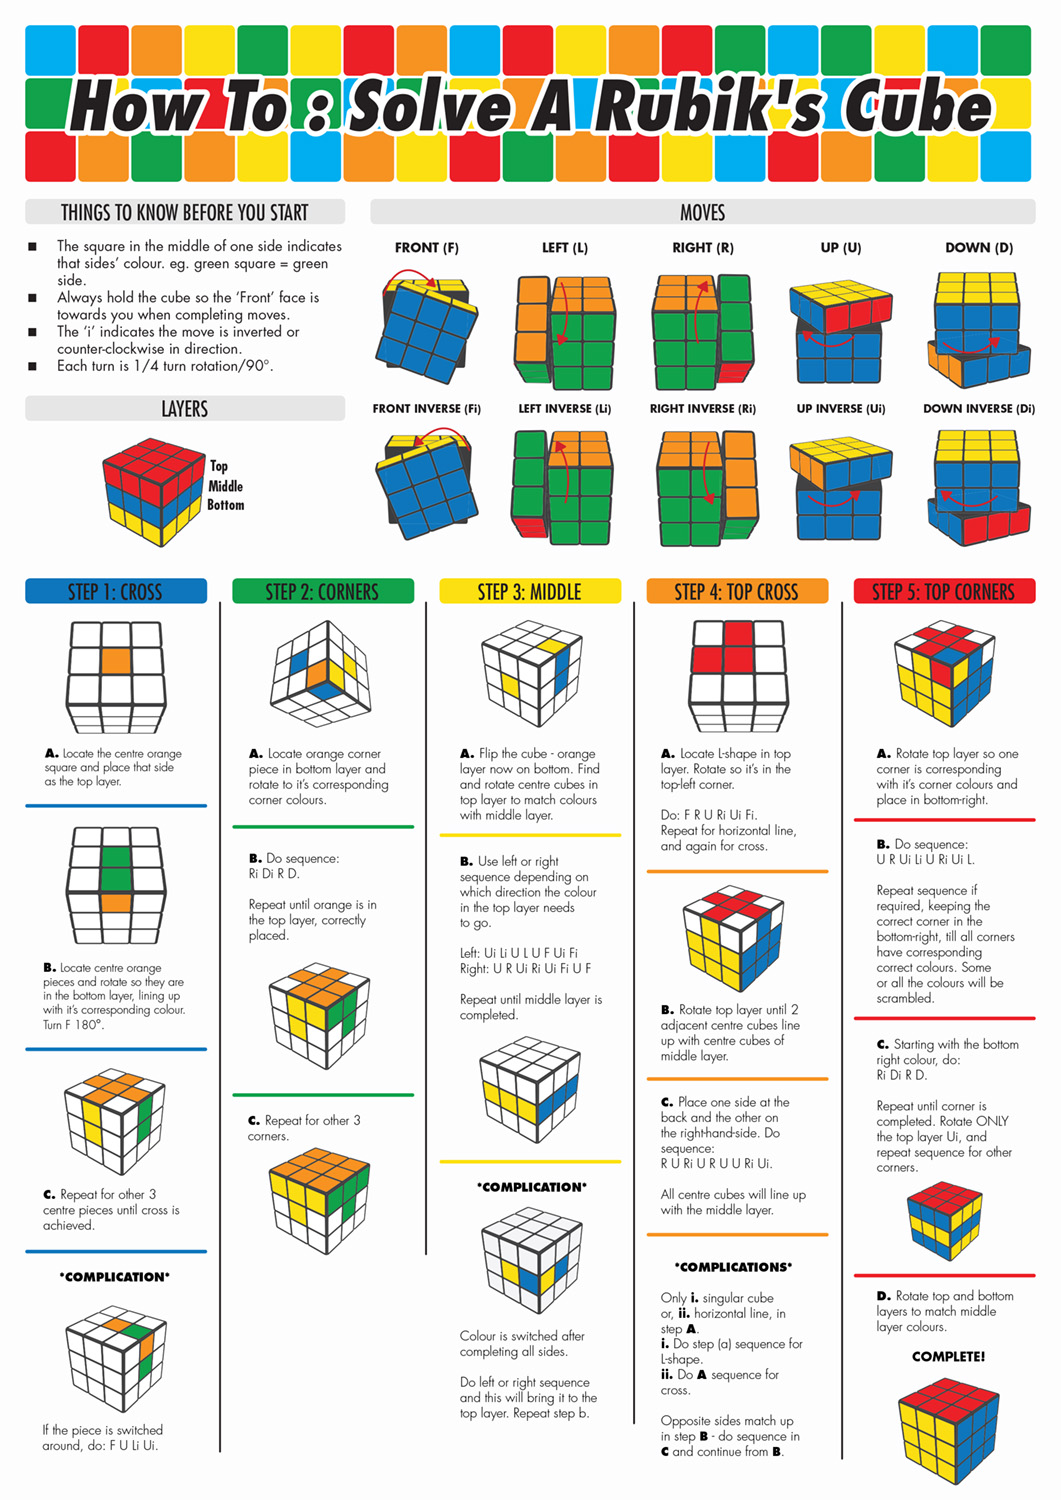
\includegraphics[width=60pt]{imgs/cubo.jpg}
\end{figure}
\end{frame}

%%%%%%%%%%%%%%%%%%%%%%%%%%%%%%%%%%%%%%%%%%%%%%%%%%%%%%%%%%%%%%%%%%%%%%%%%%%%%%%%%%%%%%%%%%%%

\begin{frame}{Introdução}{Algoritmos}
Como representar um algoritmo?
\begin{itemize}
\item Vamos usar preferencialmente pseudo-código.
\item Por vezes usaremos C/C++ ou frases em português.
\item O pseudo-código é baseado em linguagens imperativas. 
\item É ``legível'' e  independente de qualquer compliador ou arquitetura.
\end{itemize}
\end{frame}

%%%%%%%%%%%%%%%%%%%%%%%%%%%%%%%%%%%%%%%%%%%%%%%%%%%%%%%%%%%%%%%%%%%%%%%%%%%%%%%%%%%%%%%%%%%%

\begin{frame}[fragile]{Algoritmos}{Pseudo-código x Código em C}
\begin{columns}[T] % align columns
\begin{column}{.48\textwidth}
\color{red}\rule{\linewidth}{4pt}
\begin{algorithm}[H]
\caption{Pseudo-código} 
\label{pseudocodigo}
\Inicio{
  $k \leftarrow 0$ \\
  \Repita{($ k \geq 10$)} {
  \Para {($j \leftarrow0  \textrm{ até } n - 1$)} {
    $i \leftarrow j - 1$ \\
    \Enqto {($i > 0$)} {
	$i \leftarrow i - 1$ \\
    }
  }
  $k \leftarrow k + 1;$ \\
  }
}
\end{algorithm}
\end{column}%
\hfill%
\begin{column}{.48\textwidth}
\color{blue}\rule{\linewidth}{4pt}
Código em C
\begin{lstlisting}
int main() {
  int k = 0, j;
  do {
    for (j = 0; j < n; j++) {
      int i = j - 1;
      while (i > 0) 
        i = i - 1;
    }
    k = k + 1;
  } while (k < 10);
}
\end{lstlisting}
\end{column}%
\end{columns}
\end{frame}

%%%%%%%%%%%%%%%%%%%%%%%%%%%%%%%%%%%%%%%%%%%%%%%%%%%%%%%%%%%%%%%%%%%%%%%%%%%%%%%%%%%%%%%%%%%%
\section{Tempo de Processamento}
%%%%%%%%%%%%%%%%%%%%%%%%%%%%%%%%%%%%%%%%%%%%%%%%%%%%%%%%%%%%%%%%%%%%%%%%%%%%%%%%%%%%%%%%%%%%

\begin{frame}{Tempo de Processamento}{Algoritmos}
Como escolher o melhor algoritmo?
\begin{block}{Tempo de Processamento}
Um algoritmo que realiza uma tarefa em 10 horas é melhor que outro que realiza em 10 dias.
\end{block}
\begin{block}{Quantidade de memória necessária}
Um algoritmo que usa 1MB de memória RAM é melhor que outro que usa 1GB.
\end{block}
\end{frame}

%%%%%%%%%%%%%%%%%%%%%%%%%%%%%%%%%%%%%%%%%%%%%%%%%%%%%%%%%%%%%%%%%%%%%%%%%%%%%%%%%%%%%%%%%%%%

\begin{frame}{Tempo de Processamento}
\begin{itemize}
\item Medir o tempo gasto por um algoritmo {\bf não} é uma boa opção.
\begin{itemize}
\item Depende do compilador. 
\begin{itemize}
\item Pode preferir algumas construções ou otimizar melhor
\end{itemize}
\item Depende do hardware
\begin{itemize}
\item GPU vs. CPU
\item Desktop vs. smartphone
\end{itemize}
\end{itemize}
\item A solução é estudar o número de vezes que operações são executadas.
\end{itemize}
\end{frame}

%%%%%%%%%%%%%%%%%%%%%%%%%%%%%%%%%%%%%%%%%%%%%%%%%%%%%%%%%%%%%%%%%%%%%%%%%%%%%%%%%%%%%%%%%%%%

\begin{frame}{Tempo de Processamento}
\begin{itemize}
\item Precisamos de um padrão para contagem das operações:
\begin{itemize}
\item Cada operação simples (ex: +, -, /, *, Se) demora 1 passo.
\item Laços de repetição e funções não são instruções simples!
\item Cada acesso à memória custa também 1 passo
\end{itemize}
\item Ao medir o tempo de execução contando o número de passos definimos uma função: $T (n)$.
\item As operações estão simplificadas, mas mesmo assim isto é útil
\item Ex: somar dois inteiros não custa o mesmo que dividir dois reais, mas esses valores, numa visão global, não são importantes.
\end{itemize}
\end{frame}

%%%%%%%%%%%%%%%%%%%%%%%%%%%%%%%%%%%%%%%%%%%%%%%%%%%%%%%%%%%%%%%%%%%%%%%%%%%%%%%%%%%%%%%%%%%%
\section{Exemplo: Soma Vetor}
%%%%%%%%%%%%%%%%%%%%%%%%%%%%%%%%%%%%%%%%%%%%%%%%%%%%%%%%%%%%%%%%%%%%%%%%%%%%%%%%%%%%%%%%%%%%

\begin{frame}[fragile]{Exemplo}{Um problema exemplo - Soma}
Exemplo: Algoritmo que soma os elementos de um vetor.
\begin{columns}[T] % align columns
\begin{column}{.68\textwidth}
\scalebox{0.95}{
\begin{algorithm}[H]
\caption{SomaVetor} 
\label{SomaVetor}
\Entrada{Vetor $V[0..n-1]$, tamanho $n$}
\Saida{Soma dos elementos de um vetor}
\Inicio{
	$soma \leftarrow 0 $  \\ 
	\Para {($i \leftarrow 0$ até $n-1$)} {
          $soma \leftarrow soma + V[ i ]$\\
	}
	\Retorna soma
}
\end{algorithm}
}
\end{column}%
\hfill%
\begin{column}{.28\textwidth}
\begin{verbatim}
Nº execuções


Linha 2: 1
Linha 3: n+1
Linha 4: n
Linha 5: 1
\end{verbatim}
\end{column}%
\end{columns}

Tempo de Processamento de SomaVetor:\\
$T(n) = 1 + (n+1) + n + 1 = 2n+3$
\end{frame}

%%%%%%%%%%%%%%%%%%%%%%%%%%%%%%%%%%%%%%%%%%%%%%%%%%%%%%%%%%%%%%%%%%%%%%%%%%%%%%%%%%%%%%%%%%%%

\begin{frame}{Exemplo}{Tempo de Processamento}
\begin{itemize}
\item Análise de complexidade é feita em função de $n$:
\begin{itemize}
\item $n$ indica o tamanho da entrada.
\item Número de elementos no vetor.
\item Número de vértices num grafo.
\item Número de linhas de uma matriz.
\end{itemize}
\item Diferentes entradas podem ter custo diferente:
\begin{itemize}
\item Melhor caso
\item Pior caso
\item Caso médio
\end{itemize}
\end{itemize}
\end{frame}

%%%%%%%%%%%%%%%%%%%%%%%%%%%%%%%%%%%%%%%%%%%%%%%%%%%%%%%%%%%%%%%%%%%%%%%%%%%%%%%%%%%%%%%%%%%%
\section{Exemplo: Busca Vetor}
%%%%%%%%%%%%%%%%%%%%%%%%%%%%%%%%%%%%%%%%%%%%%%%%%%%%%%%%%%%%%%%%%%%%%%%%%%%%%%%%%%%%%%%%%%%%

\begin{frame}{Exemplo}{Busca Vetor}
Faça a análise do tempo de execução de um algoritmo que realiza a busca de um elemento em um vetor. O algoritmo recebe como entrada um vetor de tamanho $n$ e retorna a posição que o elemento se encontra no vetor. Caso não encontre o elemento no vetor, o algoritmo deve retornar -1.
\end{frame}

%%%%%%%%%%%%%%%%%%%%%%%%%%%%%%%%%%%%%%%%%%%%%%%%%%%%%%%%%%%%%%%%%%%%%%%%%%%%%%%%%%%%%%%%%%%%

\begin{frame}[fragile]{Exemplo}{Um problema exemplo - Busca Vetor}
Exemplo: Algoritmo que busca um elemento em um vetor.
\begin{columns}[T] % align columns
\begin{column}{.68\textwidth}
\scalebox{0.95}{
\begin{algorithm}[H]
\caption{BuscaVetor} 
\label{BuscaVetor}
\Entrada{Vetor $V[0..n-1]$, tamanho $n$, elemento $x$}
\Saida{Posição do elemento $x$ no vetor V.}
\Inicio{
    $i \leftarrow 0$ \\
	\Enqto {($i < n$)} {
		\Se {($V[i] = x$)} {
			\Retorna $i$ \\
		}
          $i \leftarrow i + 1$\\
	}
	\Retorna $-1$
}
\end{algorithm}
}
\end{column}%
\hfill%
\begin{column}{.28\textwidth}
\begin{verbatim}
Nº execuções
Pior Caso|Melhor Caso
Linha 2: 1
Linha 3: n + 1 | 1       
Linha 4: n | 1
Linha 5: 0 | 1
Linha 6: n | 0      
Linha 7: 1 | 0
\end{verbatim}
\end{column}%
\end{columns}
\end{frame}

%%%%%%%%%%%%%%%%%%%%%%%%%%%%%%%%%%%%%%%%%%%%%%%%%%%%%%%%%%%%%%%%%%%%%%%%%%%%%%%%%%%%%%%%%%%%

\begin{frame}[fragile]{Exemplo}{Um problema exemplo - Busca Vetor}
\begin{itemize}
\item Melhor caso: $T(n) = 1 + 1 + 1 + 1 + 0 + 0= 4$
\item Pior caso: $T(n) = 1 + (n + 1) + n + 0 + n + 1 = 3n + 3$
\item Caso Médio:
\begin{itemize}
\item As linhas 3, 4 e 6 são executadas em média:
\begin{itemize}
\item $L3 = \frac{(n + 2)}{2} = \frac{n}{2} + 1$
\item $L4 = \frac{n+1}{2}$
\item $L6 = \frac{n}{2}$
\end{itemize}
\item $L5$ é executado 1 vez e $L7$ não é executada.
\item $T(n) = 1 + (\frac{n}{2} + 1) + (\frac{n+1}{2}) + 1 + \frac{n}{2} + 0 = \frac{3n}{2} + \frac{7}{2}$
\end{itemize}
\end{itemize}
\end{frame}

%%%%%%%%%%%%%%%%%%%%%%%%%%%%%%%%%%%%%%%%%%%%%%%%%%%%%%%%%%%%%%%%%%%%%%%%%%%%%%%%%%%%%%%%%%%%
\section{Exemplo: Elemento Máximo}
%%%%%%%%%%%%%%%%%%%%%%%%%%%%%%%%%%%%%%%%%%%%%%%%%%%%%%%%%%%%%%%%%%%%%%%%%%%%%%%%%%%%%%%%%%%%

\begin{frame}{Exemplo}{Elemento Máximo}
Faça a análise do tempo de execução de um algoritmo que realiza a busca do {\bf maior} elemento em um vetor. O algoritmo recebe como entrada um vetor de tamanho $n$ e retorna o valor do maior elemento presente no vetor.
\end{frame}

%%%%%%%%%%%%%%%%%%%%%%%%%%%%%%%%%%%%%%%%%%%%%%%%%%%%%%%%%%%%%%%%%%%%%%%%%%%%%%%%%%%%%%%%%%%%

\begin{frame}[fragile]{Exemplo}{Um problema exemplo - Max}
Exemplo: Algoritmo que encontra o elemento máximo de um vetor.
\begin{columns}[T] % align columns
\begin{column}{.68\textwidth}
\scalebox{0.95}{
\begin{algorithm}[H]
\caption{MaxVetor} 
\label{MaxVetor}
\Entrada{Vetor $V[0..n-1]$, tamanho $n$}
\Saida{Elemento máximo do vetor}
\Inicio{
	$max \leftarrow V[ 0 ]$  \\ 
	\Para {($i \leftarrow 1$ até $n-1$)} {
	  \Se {( $V[ i ]  > max$ ) } {
          $max \leftarrow V[ i ]$\\
        }
	}
	\Retorna max
}
\end{algorithm}
}
\end{column}%
\hfill%
\begin{column}{.28\textwidth}
\begin{verbatim}
Nº execuções

Pior Caso|Melhor Caso
Linha 2: 1
Linha 3: n
Linha 4: n-1
Linha 5: n-1|0

Linha 6: 1
\end{verbatim}
\end{column}%
\end{columns}
\begin{itemize}
\item Melhor caso: $T(n) = 1 + n + (n-1) + 0 + 1 = 2n+1$
\item Pior caso: $T(n) = 1 + n + (n-1) + (n-1) + 1 = 3n$
\item Caso Médio: a linha 5 executa $\frac{n-1}{2}$ vezes. $T(n)= \frac{5n+1}{2}$
\end{itemize}
\end{frame}

%%%%%%%%%%%%%%%%%%%%%%%%%%%%%%%%%%%%%%%%%%%%%%%%%%%%%%%%%%%%%%%%%%%%%%%%%%%%%%%%%%%%%%%%%%%%
\section{Exemplo: Elemento Máximo e Mínimo}
%%%%%%%%%%%%%%%%%%%%%%%%%%%%%%%%%%%%%%%%%%%%%%%%%%%%%%%%%%%%%%%%%%%%%%%%%%%%%%%%%%%%%%%%%%%%

\begin{frame}{Exemplo}{Elemento Máximo e Mínimo}
Faça a análise do tempo de execução de um algoritmo que realiza a busca do {\bf maior} e do {\bf menor} elemento em um vetor. O algoritmo recebe como entrada um vetor de tamanho $n$ e retorna dois valores: o maior e o menor elemento presentes no vetor.
\end{frame}

%%%%%%%%%%%%%%%%%%%%%%%%%%%%%%%%%%%%%%%%%%%%%%%%%%%%%%%%%%%%%%%%%%%%%%%%%%%%%%%%%%%%%%%%%%%%

\begin{frame}[fragile]{Exemplo}{Um problema exemplo - MaxMin1}
Exemplo: Algoritmo que encontra os valores máximo e minimo em um vetor.
\begin{columns}[T] % align columns
\begin{column}{.68\textwidth}
\scalebox{0.95}{
\begin{algorithm}[H]
\caption{MaxMin1} 
\label{MaxMin1}
\Entrada{Vetor $V[0..n-1]$, tamanho $n$}
\Saida{Elemento máximo e mínimo do vetor}
\Inicio{
	$max \leftarrow V[ 0 ]$  \\ 
	$min \leftarrow V[ 0 ]$  \\ 
	\Para {($i \leftarrow 1$ até $n-1$)} {
	  \Se {( $V[ i ]  > max$ ) } {
          $max \leftarrow V[ i ]$\\
        }
	  \Se {( $V[ i ]  < min$ ) } {
          $min \leftarrow V[ i ]$\\
        }        
	}
	\Retorna (max,min)
}
\end{algorithm}
}
\end{column}%
\hfill%
\begin{column}{.28\textwidth}
\begin{verbatim}
Nº execuções

Pior Caso|Melhor Caso
Linha 2 e 3: 1

Linha 4: n
Linha 5: n-1
Linha 6: n-1|0
Linha 7: n-1
Linha 8: 0|n-1
Linha 9: 1
\end{verbatim}
\end{column}%
\end{columns}
\end{frame}
	
%%%%%%%%%%%%%%%%%%%%%%%%%%%%%%%%%%%%%%%%%%%%%%%%%%%%%%%%%%%%%%%%%%%%%%%%%%%%%%%%%%%%%%%%%%%%

\begin{frame}{Exemplo}{Um problema exemplo - MaxMin1}
\begin{itemize}
\item Melhor caso: $T(n) = 2 + n + 3(n-1) + 0 + 1 = 4n$
\item Pior caso: $T(n) = 4n$
\item Caso Médio: $T(n) = 4n$
\end{itemize}
\end{frame}
%%%%%%%%%%%%%%%%%%%%%%%%%%%%%%%%%%%%%%%%%%%%%%%%%%%%%%%%%%%%%%%%%%%%%%%%%%%%%%%%%%%%%%%%%%%%

\begin{frame}[fragile]{Exemplo}{Um problema exemplo - MaxMin1}
\begin{columns}[T] % align columns
\begin{column}{.5\textwidth}
Uma melhora no algoritmo MaxMin1: 
\begin{itemize}
\item Não é necessário executar a linha 7 se a expressão da linha 5 for {\bf verdadeira}.
\item Ou seja, se $V[i] > max$ , então não precisamos checar se $V[i] < min$.
\end{itemize}
\end{column}%

\hfill%

\begin{column}{.5\textwidth}
\scalebox{0.8}{
\begin{algorithm}[H]
\caption{MaxMin1} 
\label{MaxMin1}
\Entrada{Vetor $V[0..n-1]$, tamanho $n$}
\Saida{Elemento máximo e mínimo do vetor}
\Inicio{
	$max \leftarrow V[ 0 ]$  \\ 
	$min \leftarrow V[ 0 ]$  \\ 
	\Para {($i \leftarrow 1$ até $n-1$)} {
	  \Se {( $V[ i ]  > max$ ) } {
          $max \leftarrow V[ i ]$\\
        }
	  \Se {( $V[ i ]  < min$ ) } {
          $min \leftarrow V[ i ]$\\
        }        
	}
	\Retorna (max,min)
}
\end{algorithm}
}
\end{column}%
\end{columns}
\end{frame}
	
	
%%%%%%%%%%%%%%%%%%%%%%%%%%%%%%%%%%%%%%%%%%%%%%%%%%%%%%%%%%%%%%%%%%%%%%%%%%%%%%%%%%%%%%%%%%%%

\begin{frame}[fragile]{Exemplo}{Um problema exemplo - MaxMin2}
\begin{columns}[T] % align columns
\begin{column}{.68\textwidth}
\scalebox{0.95}{
\begin{algorithm}[H]
%  \scriptsize
\caption{MaxMin2} 
\label{MaxMin2}
\Entrada{Vetor $V[0..n-1]$, tamanho $n$}
\Saida{Elemento máximo e mínimo do vetor}
\Inicio{
	$max \leftarrow V[ 0 ]$  \\ 
	$min \leftarrow V[ 0 ]$  \\ 
	\Para {($i \leftarrow 1$ até $n-1$)} {
	  \Se {( $V[ i ]  > max$ ) } {
          $max \leftarrow V[ i ]$\\
        }
	  \Senao {
	  	\Se {( $V[ i ]  < min$ ) } {
          		$min \leftarrow V[ i ]$\\
          	}
	  }        
	}
	\Retorna (max,min)
}
\end{algorithm}
}
\end{column}%
\hfill%
\begin{column}{.28\textwidth}
\begin{verbatim}
Nº execuções
Pior Caso|Melhor Caso
Linha 2 e 3: 1

Linha 4: n
Linha 5: n-1
Linha 6: n-1|0
Linha 7: -
Linha 8: 0|n-1
Linha 9: 0|n-1
Linha 10: 1
\end{verbatim}
\end{column}%
\end{columns}
\end{frame}
	
%%%%%%%%%%%%%%%%%%%%%%%%%%%%%%%%%%%%%%%%%%%%%%%%%%%%%%%%%%%%%%%%%%%%%%%%%%%%%%%%%%%%%%%%%%%%

\begin{frame}{Exemplo}{Um problema exemplo - MaxMin2}
\begin{itemize}
\item Melhor caso: ocorre quando o vetor está em ordem crescente.
\begin{itemize}
\item Nesse caso, a linha 6 é executada $n-1$ vezes, e as linhas 6, 8 e 9 zero vezes.
\item $T(n) = 2 + n + 2(n-1) + 1 = 3n+1$
\end{itemize}
\item Pior caso: ocorre quando o vetor está em ordem decrescente.
\begin{itemize}
\item Nesse caso, as linhas 6 a 9 são executadas $n-1$ vezes.
\item $T(n) = 2 + n + 3(n-1) + 1 = 4n$
\end{itemize}
\item Caso Médio: ocorre quando $V[i]$ é maior que $max$ metade das vezes. 
\begin{itemize}
\item Isso faz com que as linhas 6, 8 e 9 sejam executadas $\frac{(n-1)}{2}$ vezes.
\end{itemize}
\begin{eqnarray}
T(n) &=& 2 + n + (n-1) + \frac{3(n-1)}{2} + 1 = 4n\nonumber \\
     &=& 2n + 3n/2 +2 -1 -3/2 + 1\nonumber \\
     &=& \frac{(7n - 1)}{2}\nonumber
\end{eqnarray}     
\end{itemize}
\end{frame}

%%%%%%%%%%%%%%%%%%%%%%%%%%%%%%%%%%%%%%%%%%%%%%%%%%%%%%%%%%%%%%%%%%%%%%%%%%%%%%%%%%%%%%%%%%%%

\begin{frame}{Exemplo}{Um problema exemplo - MaxMin3}
\begin{columns}[T] % align columns
\begin{column}{.28\textwidth}
Dá pra fazer melhor?
\begin{figure}[!ht]
  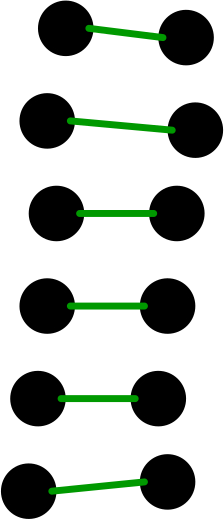
\includegraphics[width=60pt]{imgs/maxmin3.png}
\end{figure}
\end{column}%
\hfill%
\begin{column}{.68\textwidth}
\begin{itemize}
\item Comparar elementos par-a-par
\item Custo: $\frac{n}{2}$ comparações
\end{itemize}
\end{column}%
\end{columns}
\end{frame}

%%%%%%%%%%%%%%%%%%%%%%%%%%%%%%%%%%%%%%%%%%%%%%%%%%%%%%%%%%%%%%%%%%%%%%%%%%%%%%%%%%%%%%%%%%%%

\begin{frame}{Exemplo}{Um problema exemplo - MaxMin3}
\begin{columns}[T] % align columns
\begin{column}{.28\textwidth}
Dá pra fazer melhor?
\begin{figure}[!ht]
  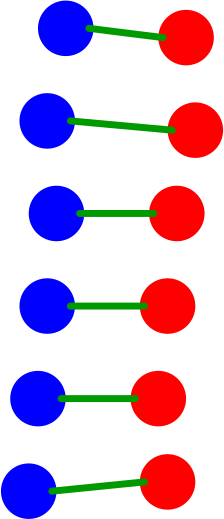
\includegraphics[width=60pt]{imgs/maxmin3_1.png}
\end{figure}
\end{column}%
\hfill%
\begin{column}{.68\textwidth}
\begin{itemize}
\item Comparar elementos par-a-par
\begin{itemize}
\item Custo: n/2 comparações
\end{itemize}
\item Elementos vermelhos são maiores ({\it biggers}) que os azuis
\item Encontrar o máximo entre os elementos vermelhos
\begin{itemize}
\item Custo: n/2 comparações
\end{itemize}
\item Elementos azuis são menores ({\it smallers}) que os vermelhos
\item Encontrar o mínimo entre os elementos azuis
\begin{itemize}
\item Custo: n/2 comparações
\end{itemize}
\end{itemize}
\end{column}%
\end{columns}
\end{frame}

%%%%%%%%%%%%%%%%%%%%%%%%%%%%%%%%%%%%%%%%%%%%%%%%%%%%%%%%%%%%%%%%%%%%%%%%%%%%%%%%%%%%%%%%%%%%

\begin{frame}[fragile]{Exemplo}{Um problema exemplo - MaxMin3}
\begin{columns}[T] % align columns
\begin{column}{.58\textwidth}
\scalebox{0.75}{
\begin{algorithm}[H]
\caption{MaxMin3} 
\label{MaxMin3}
\Entrada{Vetor $V[0..n-1]$, tamanho $n$}
\Saida{Elemento máximo e mínimo do vetor}
\Inicio{
	$max \leftarrow -\infty$  \\ 
	$min \leftarrow \infty$  \\ 
	\Para {($i \leftarrow 0$ até $n-1$ com $i\leftarrow i + 2$)} {
	  \Se {( $V[ i ]  < V[ i + 1]$ ) } {
          \color{blue}$s \leftarrow i$;
          \color{red}$b \leftarrow i+1$\\
        }
	  \Senao {
          \color{blue}$s \leftarrow i+1$;
          \color{red}$b \leftarrow i$\\	  
        }        
        \color{blue}\Se{($V[ s ] < min$)} {
        	\color{blue}$min \leftarrow V[ s ]$\\
	   }
        \color{red}\Se {($V[ b ] > max$)} {
        	\color{red}$max \leftarrow V[ b ]$\\
        }
	}
	\Retorna (max,min)
}
\end{algorithm}
}
\end{column}%
\hfill%
\begin{column}{.38\textwidth}
\begin{verbatim}
Nº execuções
Pior Caso|Melhor Caso
L2 e L3: 1

L4:n/2 + 1
L5: n/2
L6: 2x n/2|n/4
L7: -
L8: 2 x 0|n/4
L9 e 11: 2x n/2
L10 e L12: 2x 1| n/2
L13: 1
\end{verbatim}
\end{column}%
\end{columns}
\end{frame}

%%%%%%%%%%%%%%%%%%%%%%%%%%%%%%%%%%%%%%%%%%%%%%%%%%%%%%%%%%%%%%%%%%%%%%%%%%%%%%%%%%%%%%%%%%%%

\begin{frame}{Exemplo}{Um problema exemplo - MaxMin3}
\begin{itemize}
\item Pior caso:
\begin{itemize}
\item Linhas 10 e 12 sempre são executadas (L10 e L12 executam $\frac{n}{2}$ vezes).
\item Elementos azuis em ordem decrescente.
\item Elementos vermelhos em ordem crescente.
\item Ex. [\color{blue} 4 \color{red} 5 \color{blue} 3 \color{red} 6 \color{blue} 2 \color{red} 7 \color{blue} 1 \color{red} 8 \color{blue} 0 \color{red} 9]
\end{itemize}
\item Melhor caso:
\begin{itemize}
\item Linhas 10 e 12 são executadas uma única vez (L10 e L12 executam 1 vez cada).
\item Elementos azuis em ordem crescente
\item Elementos vermelhos em ordem decrescente
\item Ex. [\color{blue} 0 \color{red} 9 \color{blue} 1 \color{red} 8 \color{blue} 2 \color{red} 7 \color{blue} 3 \color{red} 6 \color{blue} 4 \color{red} 5]
\end{itemize}
\item Caso médio:
\begin{itemize}
\item Linhas 10 e 12 são executadas em média $\frac{n}{4}$ vezes.
\end{itemize}
\end{itemize}
\end{frame}

%%%%%%%%%%%%%%%%%%%%%%%%%%%%%%%%%%%%%%%%%%%%%%%%%%%%%%%%%%%%%%%%%%%%%%%%%%%%%%%%%%%%%%%%%%%%

\begin{frame}{Exemplo}{Um problema exemplo - MaxMin3}
\begin{table}[]
\centering
\caption{Custo MaxMin3}
\label{Custo MaxMin3}
% \scalebox{0.6}{
\begin{tabular}{c|ccc}
Linhas  &  Melhor  &  Pior  &  Médio  \\
\hline
2 e 3   & 2            &    2    &  2 \\
4       & $\frac{n}{2} + 1$  & $\frac{n}{2} + 1$     & $\frac{n}{2} + 1$ \\
5       & $\frac{n}{2}$       & $\frac{n}{2}$        & $\frac{n}{2}$  \\
6       & $2\frac{n}{2}$ &$2\frac{n}{2}$  & $2\frac{n}{4}$  \\
8      & 0 & 0  &  $2\frac{n}{4}$ \\
9 e 11 & $2\frac{n}{2}$ & $2\frac{n}{2}$& $2\frac{n}{2}$ \\
10 e 12 & 2 &  $2\frac{n}{2}$ &  $2\frac{n}{4}$ \\
13      & 1 & 1 & 1 \\
\end{tabular}
% }
\end{table} 

\end{frame}

%%%%%%%%%%%%%%%%%%%%%%%%%%%%%%%%%%%%%%%%%%%%%%%%%%%%%%%%%%%%%%%%%%%%%%%%%%%%%%%%%%%%%%%%%%%%

\begin{frame}{Exemplo}{Um problema exemplo - MaxMin3}
\begin{itemize}
\item Melhor caso:
\begin{eqnarray}
T(n) &=& 2 + (\frac{n}{2} + 1) + \frac{5n}{2} + 2 + 1=3n + 6\nonumber
\end{eqnarray}
\item Pior caso:
\begin{eqnarray}
T(n) &=& 2 + (\frac{n}{2} + 1) + \frac{7n}{2} + 1 = 4n + 4\nonumber
\end{eqnarray}
\item Caso médio:
\begin{eqnarray}
T(n) &=& 2 + (\frac{n}{2} + 1) + \frac{6n}{2} + 1 = \frac{7n}{2} + 4\nonumber
\end{eqnarray}
\end{itemize}
\end{frame}

%%%%%%%%%%%%%%%%%%%%%%%%%%%%%%%%%%%%%%%%%%%%%%%%%%%%%%%%%%%%%%%%%%%%%%%%%%%%%%%%%%%%%%%%%%%%

\begin{frame}{Exemplo}{Um problema exemplo - MaxMin3}
\begin{table}[]
\centering
\caption{Comparativo MaxMin}
\label{Comparativo1 MaxMin}
\begin{tabular}{c|ccc}
Algoritmo  &  Melhor Caso  &  Pior Caso  &  Caso Médio  \\
\hline
MinMax1  &   4n       &       4n   &  4n \\
MinMax2  &   3n+1     &       5n-1   &  $\frac{(7n -1)}{2}$ \\
MinMax3  &   3n+6     & 4n+4    &  $\frac{7n}{2}$+4 \\
\end{tabular}
\end{table}
\end{frame}

%%%%%%%%%%%%%%%%%%%%%%%%%%%%%%%%%%%%%%%%%%%%%%%%%%%%%%%%%%%%%%%%%%%%%%%%%%%%%%%%%%%%%%%%%%%%

\begin{frame}[fragile]{Exemplo}{Um problema exemplo - MaxMin4}
\begin{itemize}
\item O {\it melhor caso} é um pouco pior que o algoritmo MaxMin2. 
\item É possível implementar uma última melhora.
\begin{itemize}
\item Em vez de $max$ e $min$ começaram com $-\infty$ e $\infty$, basta serem inicializadas com a primeira posição do vetor e descontar essa posição do laço de repetição.
\end{itemize}
\end{itemize}
\end{frame}

%%%%%%%%%%%%%%%%%%%%%%%%%%%%%%%%%%%%%%%%%%%%%%%%%%%%%%%%%%%%%%%%%%%%%%%%%%%%%%%%%%%%%%%%%%%%

\begin{frame}[fragile]{Exemplo}{Um problema exemplo - MaxMin4}
\begin{columns}[T] % align columns
\begin{column}{.58\textwidth}
\scalebox{0.7}{
\begin{algorithm}[H]
\caption{MaxMin4} 
\label{MaxMin4}
\Entrada{Vetor $V[0..n-1]$, tamanho $n$}
\Saida{Elemento máximo e mínimo do vetor}
\Inicio{ 
        \Se {V[0] > V[1]} {
	  $max \leftarrow V[ 0 ]$; $min \leftarrow V[ 1 ]$  \\ 
	}
	\Senao {
	  $max \leftarrow V[ 1 ]$; $min \leftarrow V[ 0 ]$  \\ 	
	}
	\Para {($i \leftarrow 2$ até $n-1$ com $i\leftarrow i + 2$)} {
	  \Se {( $V[ i ]  < V[ i + 1]$ ) } {
          \color{blue}$s \leftarrow i$;
          \color{red}$b \leftarrow i+1$\\
	  }
	    \Senao {
	    \color{blue}$s \leftarrow i+1$;
	    \color{red}$b \leftarrow i$\\	  
	  }        
	  \color{blue}\Se{($V[ s ] < min$)} {
		  \color{blue}$min \leftarrow V[ s ]$\\
	    }
	  \color{red}\Se {($V[ b ] > max$)} {
		  \color{red}$max \leftarrow V[ b ]$\\
	  }
	}
	\Retorna (max,min)
}
\end{algorithm}
}
\end{column}%
\hfill%
\begin{column}{.38\textwidth}

\begin{verbatim}
Nº execuções


L2 a L5: 3

L6:(n-2)/2 + 1
L7: (n-2)/2
L8: 2x (n-2)/2|(n-2)/4
L9: -
L10: 2x 0|(n-2)/4
L11 e 13: 2x (n-2)/2
L12 e L14: 2x 1|(n-2)/2
L15: 1
\end{verbatim}
\end{column}%
\end{columns}
\end{frame}

%%%%%%%%%%%%%%%%%%%%%%%%%%%%%%%%%%%%%%%%%%%%%%%%%%%%%%%%%%%%%%%%%%%%%%%%%%%%%%%%%%%%%%%%%%%%

\begin{frame}{Exemplo}{Um problema exemplo - MaxMin4}
\begin{table}[]
\centering
\caption{Custo MaxMin4}
\label{Custo MaxMin4}
% \scalebox{0.6}{
\begin{tabular}{c|ccc}
Linhas  &  Melhor  &  Pior  &  Médio  \\
\hline
2 a 5   & 3            &    3    &  3 \\
6       & $\frac{(n-2)}{2} + 1$  & $\frac{(n-2)}{2} + 1$     & $\frac{(n-2)}{2} + 1$ \\
7       & $\frac{(n-2)}{2}$       & $\frac{(n-2)}{2}$        & $\frac{(n-2)}{2}$  \\
8       & $2\frac{(n-2)}{2}$ & $2\frac{(n-2)}{2}$  & $2\frac{(n-2)}{4}$  \\
10      & 0 & 0 &  $2\frac{(n-2)}{4}$ \\
11 e 13 & $2\frac{(n-2)}{2}$ & $2\frac{(n-2)}{2}$& $2\frac{(n-2)}{2}$ \\
12 e 14 & 2 &  $2\frac{(n-2)}{2}$ &  $2\frac{(n-2)}{4}$ \\
15      & 1 & 1 & 1 \\
\end{tabular}
% }
\end{table} 
 
\end{frame}

%%%%%%%%%%%%%%%%%%%%%%%%%%%%%%%%%%%%%%%%%%%%%%%%%%%%%%%%%%%%%%%%%%%%%%%%%%%%%%%%%%%%%%%%%%%%

\begin{frame}{Exemplo}{Um problema exemplo - MaxMin4}
\begin{itemize}
\item Melhor caso:
\begin{eqnarray}
T(n) &=& 3 + \frac{(n-2)}{2} + 1 + \frac{(n-2)}{2} + 2\frac{(n-2)}{2} + 2 \frac{(n-2)}{2} + 3\nonumber \\
     &=& 6 \frac{(n-2)}{2} + 7 = 3n+1\nonumber 
\end{eqnarray}
\item Pior caso:
\begin{eqnarray}
T(n) &=& 3 + \frac{(n-2)}{2} + 1 + \frac{(n-2)}{2} + 2\frac{(n-2)}{2} + 4\frac{(n-2)}{2} + 1\nonumber \\
     &=& 8\frac{(n-2)}{2} + 5 = 4n -3\nonumber 
\end{eqnarray}
\item Caso médio:
\begin{eqnarray}
T(n) &=& 3 + \frac{(n-2)}{2} + 1 + 6\frac{(n-2)}{2} + 1 = 7\frac{(n-2)}{2} +5 \nonumber \\
     &=& \frac{7n}{2} -7 +5 = \frac{7n}{2} -2 \nonumber \\
\end{eqnarray}
\end{itemize}
\end{frame}

%%%%%%%%%%%%%%%%%%%%%%%%%%%%%%%%%%%%%%%%%%%%%%%%%%%%%%%%%%%%%%%%%%%%%%%%%%%%%%%%%%%%%%%%%%%%

\begin{frame}{Exemplo}{Um problema exemplo - MaxMin4}
\begin{table}[]
\centering
\caption{Comparativo MaxMin}
\label{Comparativo2 MaxMin}
\begin{tabular}{c|ccc}
Algoritmo  &  Melhor Caso  &  Pior Caso  &  Caso Médio  \\
\hline
MinMax1  &   4n       &       4n   &  4n \\
MinMax2  &   3n+1     &       5n-1   &  $\frac{(7n -1)}{2}$ \\
MinMax3  &   3n+6     & 4n+4    &  $\frac{7n}{2}$+4 \\
MinMax4  &   3n+1     &      4n-3 &  $\frac{7n}{2}-2$ \\
\end{tabular}
\end{table}
\end{frame}

%%%%%%%%%%%%%%%%%%%%%%%%%%%%%%%%%%%%%%%%%%%%%%%%%%%%%%%%%%%%%%%%%%%%%%%%%%%%%%%%%%%%%%%%%%%%
\section{Comportamento Assintótico}
%%%%%%%%%%%%%%%%%%%%%%%%%%%%%%%%%%%%%%%%%%%%%%%%%%%%%%%%%%%%%%%%%%%%%%%%%%%%%%%%%%%%%%%%%%%%

\begin{frame}{Comportamento Assintótico}
\begin{itemize}
 \item Para valores pequenos de $n$, praticamente qualquer algoritmo custa pouco para ser executado.
 \item Logo: a escolha do algoritmo tem pouquíssima influência em problemas de tamanho pequeno.
 \item Estamos realmente interessados como o algoritmo se comporta conforme $n$ aumenta indefinidamente.
\end{itemize}
\end{frame}

%%%%%%%%%%%%%%%%%%%%%%%%%%%%%%%%%%%%%%%%%%%%%%%%%%%%%%%%%%%%%%%%%%%%%%%%%%%%%%%%%%%%%%%%%%%%

\begin{frame}
  \frametitle{FIM}
\centering
\alert{Fim}
\end{frame}	

%%%%%%%%%%%%%%%%%%%%%%%%%%%%%%%%%%%%%%%%%%%%%%%%%%%%%%%%%%%%%%%%%%%%%%%%%%%%%%%%%%%%%%%%%%%%

\begin{frame}[plain]
  \titlepage
\end{frame}

%%%%%%%%%%%%%%%%%%%%%%%%%%%%%%%%%%%%%%%%%%%%%%%%%%%%%%%%%%%%%%%%%%%%%%%%%%%%%%%%%%%%%%%%%%%%

\end{document}
